% Shared standalone design for the editable figure reconstructions.
\documentclass[tikz,border=5pt,10pt]{standalone}
\usepackage[T1]{fontenc}
\usepackage[utf8]{inputenc}
\usepackage{newpxtext,newpxmath}
\usepackage[scaled=.94]{sourcesanspro}
\usepackage{pgfplots}
\pgfplotsset{compat=1.18}
\usetikzlibrary{arrows.meta,calc,positioning,decorations.pathreplacing,
  decorations.markings,patterns,matrix,shapes.geometric,fit,backgrounds,
  intersections,angles,quotes}
\definecolor{ink}{HTML}{203746}
\definecolor{accent}{HTML}{146C78}
\definecolor{muted}{HTML}{667780}
\definecolor{signalred}{HTML}{B94B44}
\color{ink}
\tikzset{>=Latex,line width=.8pt,
  every node/.style={font=\small},
  axis/.style={->,draw=muted,line width=.5pt},
  guide/.style={draw=muted,dashed,line width=.45pt},
  curve/.style={draw=accent,line width=1pt},
  marker/.style={circle,fill=accent,inner sep=1.5pt},
  labelbox/.style={fill=white,inner sep=2pt}}

\begin{document}
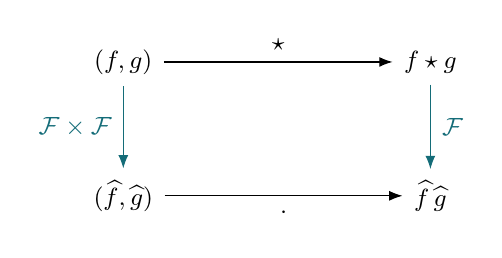
\begin{tikzpicture}[every node/.style={font=\small,inner sep=4pt}]
\node (a) at (0,0) {$(f,g)$}; \node (b) at (3.9,0) {$f\star g$};
\node (c) at (0,-1.7) {$(\widehat f,\widehat g)$}; \node (d) at (3.9,-1.7) {$\widehat f\,\widehat g$};
\draw[->] (a)--node[above] {$\star$}(b);
\draw[->] (c)--node[below] {$\cdot$}(d);
\draw[->,accent] (a)--node[left] {$\mathcal F\times\mathcal F$}(c);
\draw[->,accent] (b)--node[right] {$\mathcal F$}(d);
\end{tikzpicture}
\end{document}
